\documentclass[a4paper,
			llpt,
			solution,
			accentcolor=tud2d,
			colorbacktitle
			]
			{tudexercise}

\usepackage[utf8]{inputenc}
\usepackage[ngerman]{babel}
\usepackage{paralist}
\usepackage{amsmath}
\usepackage{pgfplots}
\usepackage{capt-of}
\pgfplotsset{compat=newest}
\usepgfplotslibrary{units}
%\usepgfplotslibrary{units}
\usepackage{xcolor}
\usepackage{caption}
%\definecolor{tud2d}{RGB}{0,78,115}
\definecolor{litegray}{gray}{0.5}
\usepackage{multirow}
\newcommand{\ze}{\end{tabular}}
\newcommand{\upd}{\begin{tabular}{c|c}}
%% deutsche Bildunterschriften
\renewcommand{\figurename}{Abbildung}
\renewcommand{\tablename}{Tabelle}
\captionsetup{labelsep=none}
\usepackage{multicol} \setlength{\multicolsep}{0pt}

\title{Lösungsvorschlag zur fünften Hausübung}
\subtitle{Einführung in Net Centric Systems und \LaTeX, Sommersemester 2015}
\subsubtitle{Max Weller, Julian Haas, Stefan Pilot}
\begin{document}
\maketitle
\section{Transport Layer}
\subsection{What is the function of the Transport Layer? Which kind of Transport Services are provided? Describe two Transport Services and name corresponding protocols and applications making use of different service types.}
Die Transportschicht stellt folgende Kommunikationsdienste zwischen Anwendungen in einem Netzwerk bereit:
\begin{enumerate}
	\item Verbindungsorientierte Kommunikation

	Ermöglicht der Anwendung, die Verbindung als Datenstrom zu verwenden. Damit muss die Anwendung sich nicht selbst um die Aufteilung der Daten in Pakete/Datagramme kümmern.
	\item Sicherstellung der Übertragungsreihenfolge

	Datenpakete werden mit einer laufenden Nummer versehen, sodass sie, selbst wenn die Reihenfolge der Pakete in unterliegenden Schichten verändert wird, der Zielanwendung in der richtigen Reihenfolge zugestellt werden können.
	\item Zuverlässigkeit
	\item Flusskontrolle
	\item Staukontrolle
	\item Multiplexing
\end{enumerate}
Das Transmission Control Protocol (TCP) bietet alle oben angegebenen Services. Es wird z.B. von Webbrowsern als Schicht unterhalb von HTTP bzw SSL verwendet, sowie bei Mailprogrammen unterhalb von IMAP. Es kommt auch bei SSH oder FTP zum Einsatz.

Das User Datagram Protocol (UDP) arbeitet verbindungslos, Anwendungen müssen also selber sog. Datagramme bilden, außerdem ist keine Zuverlässigkeit gegeben und die Übertragungsreihenfolge wird nicht sichergestellt. Es wird z.B. von Streamingdiensten, Internettelefonie und VPNs eingesetzt.


\subsection{What is the main difference between Network and Transport Layer? Why are two different layers needed?}
Die Netzwerkschicht stellt eine Verbindung zwischen zwei Hosts (Computern) her, während die Transportschicht dies zwischen zwei Anwendungen (Prozessen) auf diesen tut.

Die Aufteilung auf zwei Schichten ermöglicht das modulare Austauschen der Funktionalitäten, z.B. kann die Umstellung auf längere Hostadressen (IPv4 auf IPv6) ausschließlich in der Netzwerkschicht stattfinden, es ist keine Änderung an den Protokollen der Transportschicht (TCP, UDP) notwendig.


\subsection{What are protocol ports? What is their purpose? How can a process address a protocol port?}
Die Ports auf Transportebene bilden zusammen mit der Adresse der Netzwerkschicht eine Socketadresse, die einen bestimmten Dienst auf einem Rechner eindeutig identifizieren. Dies ermöglicht, dass mehrere Prozesse auf einem Rechner die Netzwerkverbindung nutzen.

Beim Aufbau einer Verbindung wird beim Aufruf von "connect()" neben der IP-Adresse auch der Port angegeben. Beim Warten auf eine Verbindung bindet sich der Prozess mit "bind()" an einen Port.


\section{Flow Control}
\subsection{Consider a connection with a round-trip delay of 18msec and the sender sends a packet with 2 bytes of data every 10msec. The receiver acknowledges each packet when read, but needs 10msec to read one byte of data.}
\begin{enumerate}
\item Visualize the first 50msec of this connection without a TCP connection setup.
\item Assume a TCP flow control mechanism as shown in Figure 5.1. The receiver now has a buffer of 10 bytes and received packets are acknowledged immediately. Will the flow control mechanism stop the sender? If yes, when will it stop, for how long and will the connection stabilize? Complete the table to find the answer or justify your answer briefly.
\item Assume the same setup as in (b) but this time the segment with sequence number 3 (bytes 3+4) takes a detour through the network and arrives just before the segment with sequence number 11. How will this affect the connection? Complete the table below.
\end{enumerate}
\subsection{In sliding window protocols the sender maintains a set of sequence numbers corresponding to frames that have been sent and are as yet not acknowledged. The receiver also maintains a receiving window corresponding to the frames it is permitted to accept. The sequence numbers within the sender’s window represent frames that have been sent but are not yet acknowledged. Assume there is a sliding window protocol as shown in Figure 5.2. A sender transmits 5 frames to a receiver (sequence number 0-4) using the sliding window protocol. The parties have agreed on a window size of 2. Each frame is acknowledged individually. Sending and receiving of frames generally has higher priority than producing or receiving ACKs. One station cannot send and receive at the same time. There is a transmission delay from sender to receiver of one step. Draw the sliding windows in Figure 5.2. (no transmission errors). Given is the initial state.}
\section{Sequence Numbers}
\subsection{What is the purpose of sequence numbers? What are the problems related to the use of sequence numbers?}
Sequenznummern werden genutzt, um die Reihenfolge von TCP Paketen zu bestimmen.  Ein verschicktes Paket hat dabei immer eine höhere Sequenznummer, als das zuvor verschickte Paket.
Für jedes übertragene Byte erhöht sich die Sequenznummer um 1.
Zusätzlich werden die Nummern genutzt, um ACK Nachrichten des Empfängers den jeweiligen Paketen zuzuordnen. Die Sequenznummer, die mit dem ACK übertragen wird, entspricht dabei der Sequenznummer des nächsten vom TCP Empfänger erwarteten Bytes.
\\\\s
Ein Problem, was durch die Nutzung von Sequenznummern entsteht, ist der erhöhte Aufwand: Pro TCP Paket werden 4 Byte benötigt, um die Sequenznummer mitzuschicken. Zusätzlich dazu müssen sowohl Sender als auch Empfänger immer wieder den aktuellen Stand der Sequenznummer berechnen, um die Übertragung fortsetzen zu können.
Ein weiteres Problem ist der begrenzte Zahlenraum, der für die Sequenznummern verfügbar ist. Mit einer Länge von 4 Byte (32 Bit) ergibt sich demnach eine Maximalzahl von 4.294.967.295. Nach dieser Ziffer wird die Sequenznummer wieder auf 0 gesetzt.
\subsection{Please derive an equation that calculates the time (in seconds) after which all the sequence numbers have been used in a protocol that uses x bits for the sequence numbers. Consider packets that have a length of y bytes, and a connection speed of s bits/second.}
Die Zeit nach der alle Sequenznummern "aufgebraucht" sind ergibt sich nach Anzahl der möglichen Sequenznummern/Pakete pro Sekunde.
\\\\
\centerline{
$
    \frac{s \frac{bits}{sec}}{y*8\frac{bits}{pkg}} = \frac{s}{y*8} \frac{pkg}{sec}
$
}
\\
\\

\centerline{
$\frac{2^x seqnums}{\frac{s}{y*8} \frac{pkg}{sec}} = t$ $sec$
}
\subsection{After how many seconds, would this time be for a TCP protocol while using a 20 Gbit/s connection and 15 byte packets?}
\centerline{
$\frac{2^{32} seqnums}{\frac{20*10^9}{15*8} \frac{pkg}{sec}} \approx 25,77$ $sec$
}
Es ergibt sich eine Zahl von ca. 166666666,67 gesendeten Paketen pro Sekunde. Da im TCP Header 4 Byte (32 Bit) für die Sequenznummer vorgesehen sind, ergibt sich damit, dass nach ca. 25,77 Sekunden alle möglichen Sequenznummern aufgebraucht sind (also einmal genutzt wurden).
\section{TCP and UDP}
\subsection{Name the main differences between TCP and UDP. What are the advantages and disadvantages of each protocol?}
TCP arbeitet zuverlässig und verbindungsorientiert. Eine Anwendung, die TCP benutzt, kann sich darauf verlassen, dass alle Pakete ankommen und in der richtigen Reihenfolge sind. Über eine aufgebaute TCP-Verbindung können beide Parteien miteinander kommunizieren. Dafür ist TCP vergleichsweise komplex, erzeugt einen hohen Overhead und kann größere Verzögerungen erzeugen. \\
UDP ist nicht-zuverlässig und nicht verbindungsorientiert. Pakete können in der falschen Reihenfolge oder auch gar nicht ankommen. \textcolor{red}{Eine "UDP-Verbindung" existiert nicht, UDP ist unidirektional.} Ferner ist bei UDP die automatische Bitfehlerkorrektur durch Prüfsummen optional, während sie bei TCP immer geschieht. Die Implementierung von UDP ist vergleichsweise einfach und die entstehenden Verzögerungen sind gering.

\textcolor{red}{Möglicherweise ist das für acht Punkte nicht detailliert genug...}
\subsection{State at least two reasons why UDP could be used in software development.}
Einfache Implementierung. Geringe Latenz -> gut für Multimediaanwendungen wie Musik- oder Videostreams.
\subsection{What protocols (UDP or TCP) would you use for the following scenarios? Briefly explain your decision.}
\begin{enumerate}
\item \textbf{video live streams (e.g. sport events)}: UDP. Die geringe Latenz führt zu einer verzögerungsärmeren Übertragung. Zwar leidet durch den Verlust einzelner Pakete eventuell die Qualität, bei TCP könnte es aber zu langen Verzögerungen kommen, was ungünstiger ist.
\item \textbf{an online payment system}: TCP. Selten ist die Zuverlässigkeit der Kommunikation wichtiger als bei Payment-Systemen, verzögerungsarme Übertragung ist unwichtig, die Datenmengen sind auch sehr gering.
\item \textbf{a multiplayer action video game loaded over the Internet}: Bei Spielen soll in der Regel gewährleistet sein, dass der Zustand des Spieles bei allen Spielenden zur gleichen Zeit immer gleich ist. Kommt es also bei Einzelnen zu Verzögerungen, müssen alle anderen auf diese Einzelnen warten, damit keine unfairen Situationen entstehen. Das ist ein Argument für die Verwendung von TCP. Andererseits können Verzögerungen in der Übertragung dem Spielspaß auch sehr abträglich sein, was ein Argument für UDP ist. Bei einem Spiel mit einer großen Spielerzahl würde ich UDP verwenden, weil unfaire Nachteile für einzelne hier dem Spielspaß aller geopfert werden können. Ist die Zahl der Spieler allerdings gering, kann auch TCP verwendet werden.
\end{enumerate}
\subsection{Complete the diagrams in Figure 5.3, so that the transfer of the shown data is completed successfully for the sender as well as the receiver. Assume the TCP protocol from the lecture with cumulative acknowledgements. Fill in the sequence numbers in your solution.}
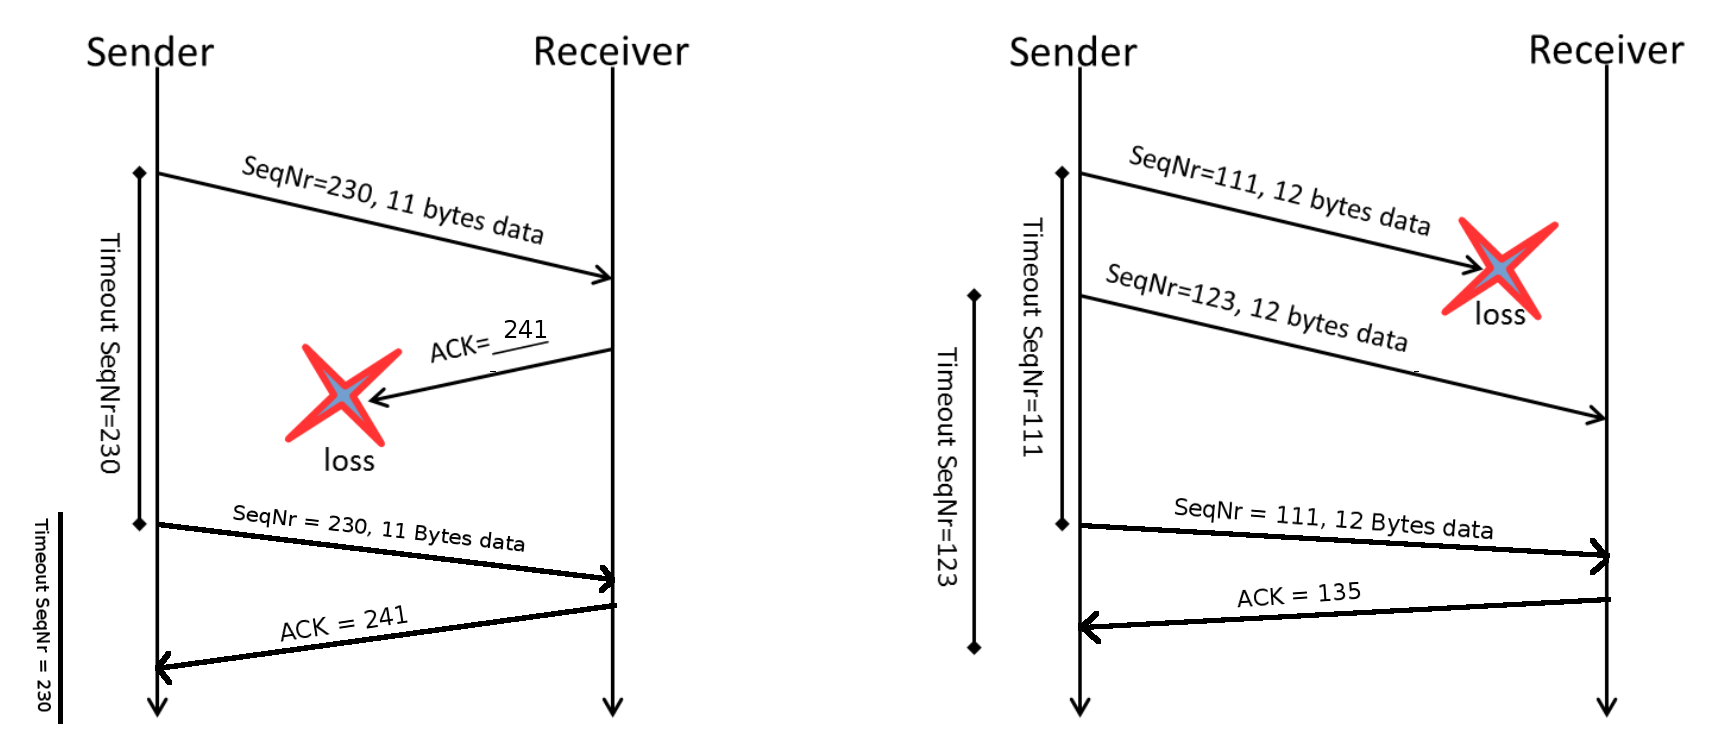
\includegraphics[width=\textwidth]{haesslon.png}
\subsection{In Figure 5.4. you can see different phases of the TCP congestion window. A TCP connection consists of the two phases slow start and congestion avoidance. In the slow start phase the threshold of the congestion window should be reached fast and a simple additive increase would take very long. The congestion window is doubled until the threshold is reached. In the congestion avoidance phase TCP switches to an additive increase of the congestion window until a timeout occurs. The congestion window is halved.}
\begin{enumerate}
\item \textbf{Which parameter is actually adapted by the congestion window?} Durch das beschriebene congestion-window-Verfahren wird die Senderate des Senders an die maximale Übertragungsrate des Netzwerks angenähert, sofern Paketverluste in der Überlastung einzelner Knoten ihre Ursache haben (und nicht etwa in der Zuverlässigkeit einzelner Verbindungen wie z.B. bei Drahtlosnetzwerken).
\item \textbf{How does a timeout occur in the depicted congestion control protocol? Describe what
happens at sender and receiver.} Ein Timeout wird dann erreicht, wenn der Sender für ein gewisses Datenpaket in einem gewissen Zeitabschnitt nach dessen Versenden kein dazu passendes ACK vom Empfänger erhält. Das kann entweder daran liegen, dass das Datenpaket den Empfänger niemals erreicht hat oder daran, dass das ACK den Sender nicht erreicht hat. Wenn der Sender nach der Timeout-Zeit kein ACK erhalten hat, sendet er das Datenpaket erneut, setzt sein Congestion Window auf 1 und halbiert das threshold, weil er davon ausgeht, dass der Paketverlust durch Netzwerkauslastung entstanden ist.
\item \textbf{What do you think why the congestion window is reduced so drastically after a timeout?}
Wird das Netzwerk stark belastet, gehen immer mehr Pakete verloren, die neu gesendet werden müssen. Arbeitet das Netzwerk an seiner Überlastungsgrenze, ist der Traffic, den es insgesamt zu bewältigen hat, also größer. Deshalb ist es sinnvoll, das congestion window stark zu senken, wenn Anzeichen vorhanden sind, dass das Netzwerk stark ausgelastet ist, um, bis der durch Paketverluste entstandene zusätzliche Traffic abgearbeitet ist.
\item \textbf{How does the task of the TCP congestion control differ from the task of flow control?}
Congestion Control berücksichtigt das gesamte (Teil-)Netz inklusive der einzelnen Komponenten (Hosts, Router etc.) und deren Prozesse und kontrolliert den gesamten Datendurchsatz.  Flow Control hingegen betrachtet einzelne (Punkt-zu-Punkt-) Verbindungen und versucht,'Überlastung langsamer Empfänger durch schnellere Sender zu vermeiden.
\end{enumerate}
\section{Three-Way Handshake}
\subsection{Given is a connection establishment using the three-way handshake as shown in Figure 5.5. which was introduced in the lecture.}
\begin{enumerate}
\item Is there a situation in which the three-way handshake fails to reliably release the connection?
Please justify your answer.
\item Describe two different alternatives how to release a connection additionally to the three-way
handshake.
\item Assume the three-way handshake protocol is reduced to the first two messages. That means
that the acknowledgement is not sent during the connection establishment. Which incorrect
behavior can occur when the connection is released after the first message is sent?
\end{enumerate}
\subsection{How does TCP release its connections? Does it avoid the problem of synchronizing the connection release? Please justify your answer briefly.}
\subsection{Figure 5.6. shows two malicious scenarios for the three-way handshake protocol using “Gesperrte Referenzen”. Describe for each of the scenarios how they violate the correct protocol. Elaborate what incorrect behavior results from this. Mark those time frames on the time axis, where the respective node assumes an established connection.}
\section{Distributed Systems}
\subsection{What are the main differences between Lamport’s and of van Renesse’s definition of distributed systems? Briefly discuss the two definitions. Give at least two counterexamples.}
\subsection{What is the purpose of a distributed system? Give at least 3 advantages and 3 disadvantages of distributed systems and briefly justify your answers.}
\subsection{Give an example for each of the different kinds of transparencies of distributed systems.}
\subsection{Describe the difference between reliability and availability. Calculate the availability and Mean Time To Failure (MTTF) for the downtimes given in Table 5.6. for the two service started on the first day of the year 2014. Argue which service is better.}
\end{document}
